\section{Zgled}

V tem poglavju bomo predstavili uporabo superimetrije na dveh preprostih primerih: eksakten izra\v cun na primeru
neskon\v cne potencialne jame in primer perturbativnega razvoja na primeru kvarti\v cnega anharmonskega oscilatorja.

\subsection{Neskon\v cna potencialna jama}

Obravnava neskon\v cne potencialne jame je standardni za\v cetni\v ski potencial. Hkrati je nekako patolo\v ski -- meja je
namre\v c neskon\v cno visoka, ostra in strma, vendar pa kljub temu obstaja supersimetri\v cni partner. Potencial bomo
omejil na $x \in [0,1]$, lastne fukcije so 

\begin{equation}
	\psi_{n-1} (x) = \sqrt{2}\sin n\pi x, \quad E_{n-1} = \frac{(n\pi)^2}{2}
		\quad n = 1, 2, 3 \ldots
\end{equation}

\ni Osnovni lastni par je $(\psi_0, E_0)$:

\begin{equation}
	\psi_0 (x) = \sqrt{2}\sin\pi x, \quad E_0 = \frac{\pi^2}{2} \neq 0.
\end{equation}

\ni Supersimetrija je v tem primeru zlomljena\footnote{Torej $E_0 \neq 0$.}, zato moramo za\v cetnemu Hamiltonianu
od\v steti energijo osnovnega stanja.

\begin{equation}
	(H - E_0)\psi_0 = (E_0 - E_0)\psi_0 =
		0\cdot\psi_0 = 0. \label{translacija}
\end{equation}

\ni Od tod lahko poi\v s\v cemo superpotencial $W(x)$ iz en.~\eqref{superpotencial}

\begin{equation}
	W(x) = -\frac{1}{\sqrt{2}} \frac{\px \sin \pi x}{\sin \pi x} = -\frac{\pi}{\sqrt{2}}\cot \pi x.
\end{equation}

\ni S pomo\v cjo en.~\eqref{v2pot} lahko poi\v s\v cemo supersimetri\v cnega partnerja neskon\v cne potencialne jame

\begin{equation}
	\tilde{V} (x) = \frac{\pi^2}{2}\bigg(\cot^2 \pi x + \frac{1}{\sin^2 \pi x}\bigg)
		= \frac{\pi^2}{2}\bigg(\frac{1}{\sin^2 \pi x} - 1\bigg), \qquad x \in [0,1],
	\label{pot-nes-jama}
\end{equation}

\ni kar o\v citno ni ve\v c neskon\v cna potencialna jama, za katero dobimo $V_1(x) = \pi^2/2$, ki pa se ravno
prikladno od\v steje s konstantno $E_0^{(1)}$ v ena\v cbi~\eqref{translacija}. Potencial $V_2$ je poseben primer
potenciala Rosen Morse I (tj. triginometri\v cna izvedenka). Kar je posebej presenetljivo, je gladkost novega potenciala.
Prej\v snji je namre\v c bila strma in ostra pregrada, ta pa je gladek.

Za izra\v cun valovnih funkcij $\tilde{\psi}_n(x)$ lahko uporabimo $a$ in $a^\dagger$, ki znane funkcije $\psi_n$
preslikata v $\tilde{\psi}_n$ in obratno. Uporabimo en.~\eqref{degenener}.
Vemo, da $\tilde{H}$ nima stanja pri $E_0$, ampak da se vezana stanja pri\v cno z $E_1$.

\begin{align}
	\tilde{\psi}_1 (x) = a\psi_1 &\propto -(\pi \cot \pi x - \px)\sin2\pi x \\
	&= \cos^2\pi x - \cos 2\pi x = \sin^2\pi x,
\end{align}

za $\tilde{\psi}_2$, tj. prvo vzbujeno stanje $\tilde{H}$, pa je

\begin{equation}
	\tilde{\psi}_2(x) \propto \sin (\pi x) \sin (2\pi x),
\end{equation}

\ni Operatorja $a$ in $a^\dagger$ seveda po pretvorbi pokvarita normalizacijo, zaradi \v cesar smo pisali sorazmernostni
znak. \v Ceprav ne moremo govoriti o bozonih in fermionih, imamo \v se vedno staro supersimetrijsko izro\v cilo:
operatorji $a$ in $a^\dagger$ simetri\v cne valovne funkcije preslikajo v anti-simetri\v cne in obratno, kar se \v se posebno
lepo vidi na sliki~\ref{sl1}.

\begin{figure}[H]
	\centering
	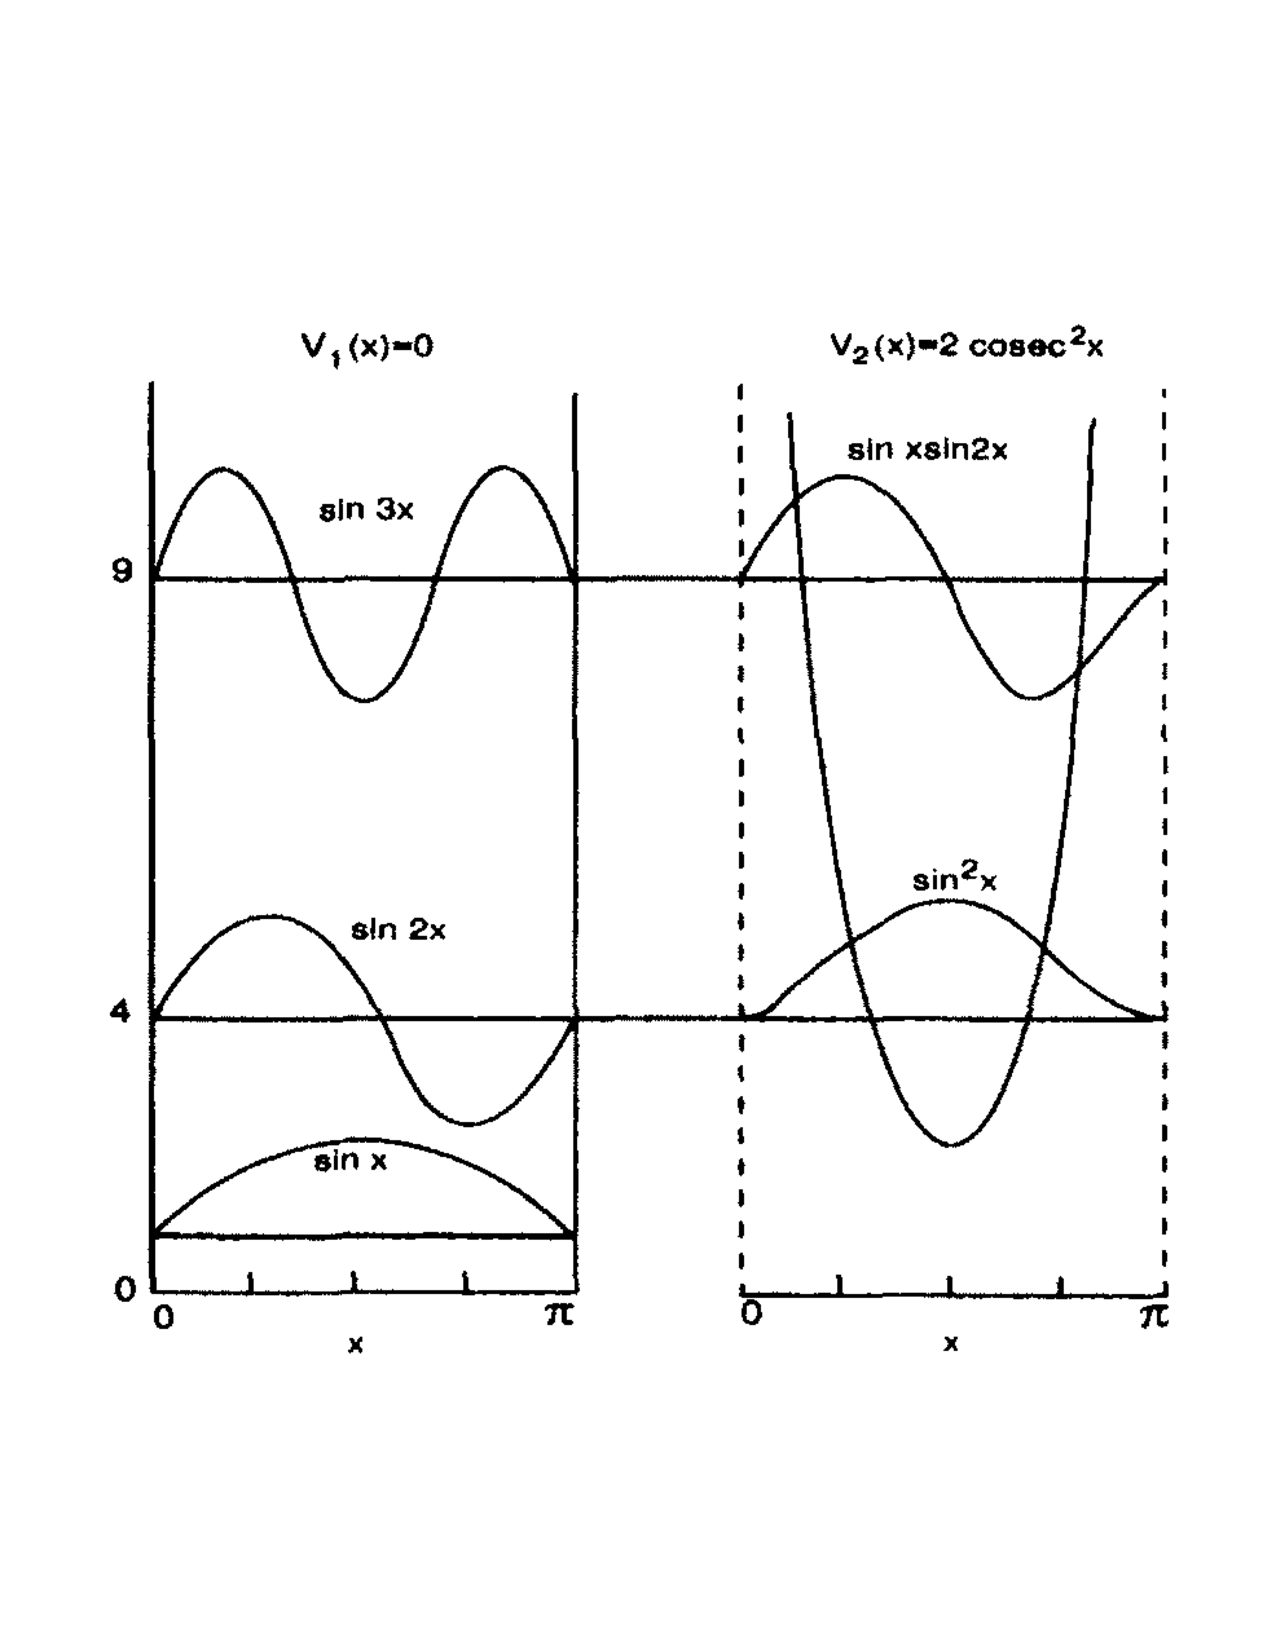
\includegraphics[height=10cm, keepaspectratio=1, trim=0cm 5cm 0cm 5cm]{pics/slika1}
	\caption{Lastna stanja operatorjev $H$ in $\tilde{H}$. $V_1$ na sliki je $V$, $V_2$ pa je $\tilde{V}$. Vidimo, kadar
		je $\psi_n$ soda funkcija, je $\tilde{\psi}_n$ liha in obratno.}
	\label{sl1}
\end{figure}

\subsection{Kvarti\v cni anharmonski oscilator}

Tega primera ne znamo re\v siti eksaktno. Re\v siti znamo samo za harmonski oscilator, zato bomo uporabili tako imenovan 
$\delta$-razvoj -- perturbacijsko metodo, ki nam pomaga aproksimirati superpotencial, prek katerega lahko potem izra\v cunamo
energije vezanih stanj in lastne funkcije.

Pri\v cnemo z dejstvom, da $V(x) = m\w^2 x^2/2$ znamo re\v siti, $V(x) = gx^4$ pa ne, zato harmonski oscilator
analiti\v cno dopolnimo do kvarti\v cnega z uvedbo parametra $\delta$, s katerim bomo dosegli $V(x;\delta_1) \sim x^2$
in $V(x;\delta_2) \sim x^4$. To naredimo tako:

\begin{equation}
	V(x;\delta) = M^{2 + \delta} x^{2 + 2\delta} - C(\delta).
	\label{anal-delta}
\end{equation}

\ni Parameter $M$ je sklopitvena konstanta, ki se lahko pri\v stuli v ra\v cun, tudi kadar imamo brezdimenzijske koli\v cine.
Skalira se ustrezno s potencialom, da so enote pravilne. Konstanta $C(\delta)$ lahko pride notri, da od\v stejemo energijo
osnovnega stanja. Tako definiran $V(x;\delta)$ nam vrne

\begin{align}
	V(x; 0) = M^2 x^2 = \frac{m\w^2}{2} x^2, \\
	V(x; 1) = M^3 x^4 = g x^4
\end{align}

\ni V prvem primeru je torej $M = \w\sqrt{m/2}$, v drugem pa $M = \sqrt[3]{g}$. Potencial $V(x;\delta)$ je analiti\v cen in
zvezen za poljuben $\delta$ na pozitivnem delu realne osi, kar pa pomeni, da lahko $V(x;\delta)$ razvijemo v poten\v cno
vrsto po potencah $\delta$:

\begin{equation}
	V(x;\delta) = M^2x^2\sum_{k = 0}^{\infty} \delta^k \bigg\{\frac{[\ln(Mx^2)]^k}{k!} - 2E_k\bigg\}
	\label{prvi}
\end{equation}

\ni Hkrati ima tudi tak potencial za vsak pozitiven $\delta$ vezana stanja, torej mu lahko priredimo superpotencial. Velja

\begin{equation}
	V(x;\delta) = W^2(x;\delta) - \koren\px W(x;\delta),
	\label{tretji}
\end{equation}

\ni kjer lahko tudi $W(x;\delta)$ prav tako razvijemo v poten\v cno vrsto:

\begin{equation}
	W(x;\delta) = \sum_{k = 0}^\infty \delta^k W_{(k)}(x).
	\label{drugi}
\end{equation}

\ni Ena\v cbo~\eqref{tretji} lahko na levi prepi\v semo z en.~\eqref{prvi}, na desni pa z en.~\eqref{drugi}. Imamo sistem
ena\v cb, razklopljen po potencah $\delta$. Za $\delta^0$ dobimo harmonski oscilator, za vi\v sji red pa dobimo \v ze
popravke k anharmonskem oscilatorju:

\begin{equation}
	W_{(0)}^2 - \koren\px W_{(0)} = M^2x^2 - 2E_0,
\end{equation}

\ni z re\v sitvami $W_{(0)} = Mx$ in $E_0 = M/2$, ki so res re\v sitve harmonskega oscilatorja. Naslednji red, tj. $\delta^1$
nam da dodatno diferencialno ena\v cbo:

\begin{equation}
	\px W_{(1)} - 2W_{(1)}W_{(0)} = -M^2x^2\ln(Mx^2) + 2E_1,
\end{equation}

ki ima re\v sitev

\begin{equation}
	W_{(1)} = -\text{e}^{Mx^2} \int_0^x \d y\ \text{e}^{-My^2}\big[M^2y^2 \ln My^2 - 2E_1\big].
\end{equation}

